\begin{spacing}{1}
    \chapter*{Abstract [L]}
\end{spacing}
\begin{wrapfigure}{r}{0.3\textwidth}
    \begin{center}
      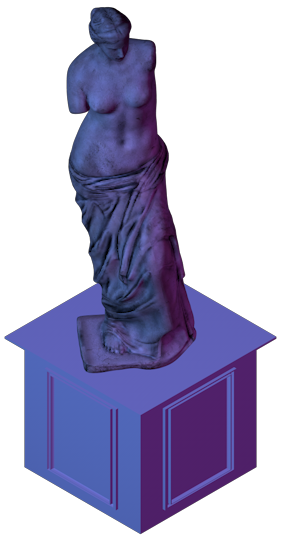
\includegraphics[width=0.2\textwidth]{pics/statue.png}
    \end{center}
\end{wrapfigure}
\setauthor{Litzlbauer Lorenz}
3D Portfolio Gallery is a web application developed by Lorenz Litzlbauer and Fabian Maar as part of their thesis. The 3D Portfolio Gallery aims to enable designers to share their design portfolio with the world in an innovative way, and to share it in a virtual three-dimensional exhibition. Designers can use 3D Portfolio Gallery to create a three-dimensional portfolio from their own media (film, photo or 3D data).



3D Portfolio Gallery is offered as a single-page application on the web and can be accessed via a web link. With a simple configuration process, the tool helps the user create the exhibition by selecting a gallery from several pre-defined layouts. Subsequently, the exhibits can be placed either automatically or manually and provided with additional information.



Visitors of the 3D gallery can move freely through the three-dimensional web exhibition and view the exhibits with different types of interaction.



For the implementation in the front end, the following frameworks are used (see \ref{txt:glos:Framework}): Angular for the single-page application and Three.js for the 3D presentation. The front-end access control and user identification in the browser uses a Json Web Token.



\newpage
\begin{spacing}{1}
    \chapter*{Zusammenfassung [L]}
\end{spacing}
\begin{wrapfigure}{r}{0.3\textwidth}
    \begin{center}
      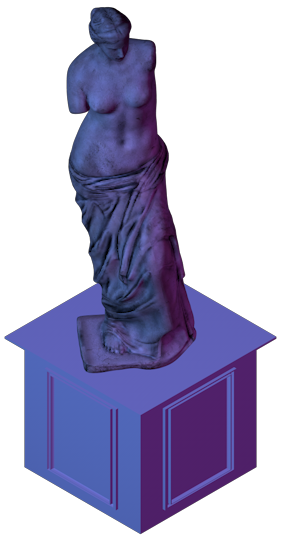
\includegraphics[width=0.2\textwidth]{pics/statue.png}
    \end{center}
\end{wrapfigure}
\setauthor{Litzlbauer Lorenz}
3D Portfolio Gallery ist eine Webapplikation, die von Lorenz Litzlbauer und Fabian Maar im Rahmen der Diplomarbeit entwickelt wurde. 3D Portfolio Gallery will Designer*innen ermöglichen, ihr Design-Portfolio auf eine innovative Art und Weise mit der Welt zu teilen und auf eine innovative Art und Weise in Form einer virtuellen dreidimensionalen Ausstellung mit der Welt zu teilen. Die Designer*innen können mithilfe von 3D Portfolio Gallery aus eigenen Medien (Film, Foto oder 3D-Daten) ein dreidimensionales Portfolio erstellen.

3D Portfolio Gallery wird als eine Single-Page-Application im Web angeboten und ist über einen Web-Link erreichbar. Das Tool unterstützt mit einem einfachen Konfigurationsprozess den User beim Erstellen der Ausstellung, indem aus mehreren vordefinierten Grundrissen eine Gallery ausgewählt wird. Anschließend können die Ausstellungsstücke entweder automatisch oder manuell platziert und mit Zusatzinformationen versehen werden.

Besucher der 3D-Gallery können sich in der dreidimensionalen Webausstellung frei bewegen und die Ausstellungsstücke mit verschiedenen Interaktionsarten anschauen.

Für die Umsetzung im Frontend werden folgende Frameworks (siehe \ref{txt:glos:Framework}) verwendet: Angular für die Single-Page-Application und Three.js für die 3D-Darstellung. In der Frontend-Zugriffkontrolle und -Useridentifikation im Browser wird die Technologie Json-Web-Token verwendet.

\chapter*{Danksagung}
Großer Dank geht an unsere Diplomarbeits-Betreuerinnen
Frau Professorin Patricia Engleitner und Frau Professorin Natascha Rammelmüller. Sie unterstützen uns im Projektverlauf durch Ihre Expertise aus den Fachgebieten Design und 3D-Modellierung und durch Ihr Feedback.
